\section{Related works}
\label{ch:relate}

Related works section

% - 讨论 client-side 的 clickstream 为什么值得研究,比较服务端搜集的 clickstream 产生的明显变化是什么。
% - 讨论现有的 client-side clickstream 研究分别是针对什么方向的,他们的结论主要是什么,都有什么样的改进空间。
% - 以前的 clickstream 只有类别级的分配模型,通过人工设计某个特定网站的马尔科夫模型来学习用户在不同类别之间的跳转概率。但当变为客户端后,数据变得更加充分,用户在一段时间内可能不局限于某个特定的网站,同时可能被其他网站干扰。
% - 这里需要讨论 searchstream 的论文


\subsection{Clickstream Behavior}

% - 这一篇是第一篇 clientside clickstream 的研究:Nils Kammenhuber, Julia Luxenburger, Anja Feldmann, and Gerhard Weikum. 2006. Web search clickstreams. In Proceedings of the 6th ACM SIGCOMM conference on Internet measurement (IMC '06). ACM, New York, NY, USA, 245-250.

% 关于时间的研究
% @inproceedings{liu2010understanding,
%   title={Understanding web browsing behaviors through Weibull analysis of dwell time},
%   author={Liu, Chao and White, Ryen W and Dumais, Susan},
%   booktitle={Proceedings of the 33rd international ACM SIGIR conference on Research and development in information retrieval},
%   pages={379--386},
%   year={2010},
%   organization={ACM}
% }


% 关于 assistent 的研究
% @article{lieberman1995letizia,
%   title={Letizia: An agent that assists web browsing},
%   author={Lieberman, Henry and others},
%   journal={IJCAI (1)},
%   volume={1995},
%   pages={924--929},
%   year={1995}
% }

\begin{figure}[H]
    \centering
    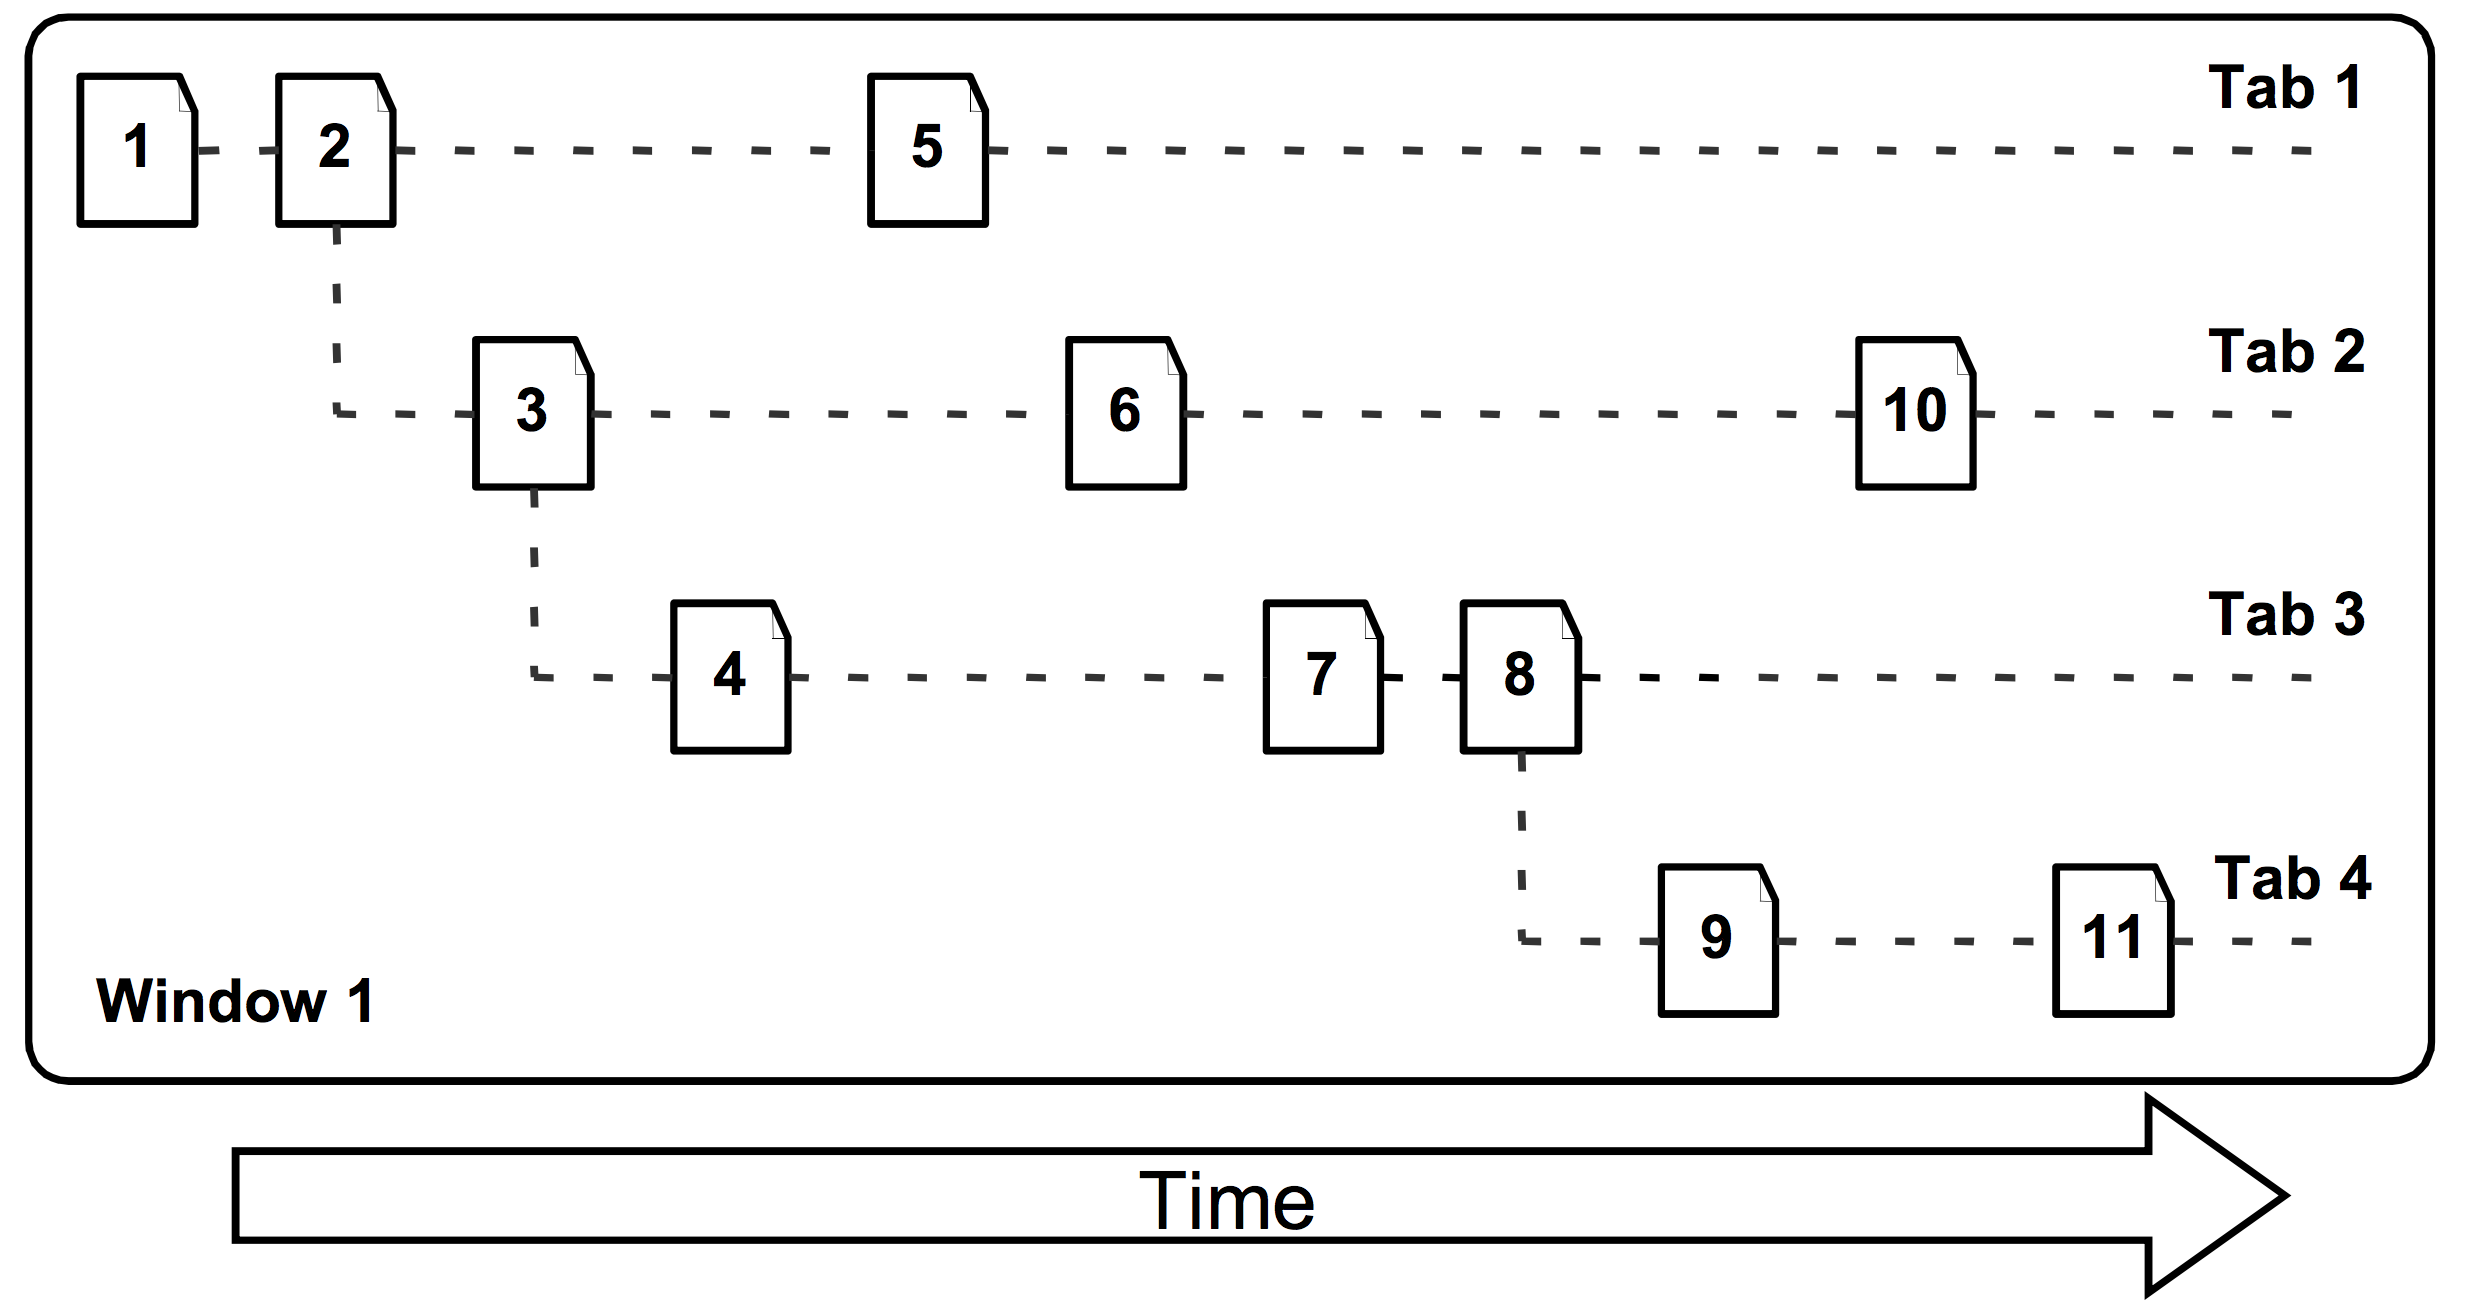
\includegraphics[width=0.7\textwidth]{figures/branching-and-backtracking}
    \caption{Parallel browsing behavior: branching phenomenon \cite{huang2010parallel}}
    \label{fig:backtrace}
\end{figure}

Huang et al. \cite{huang2012no} also discovered the behavior of backtracking browsing
however the branching

\subsection{Theory of Information Seeking Behavior}
\label{sec:info-seek}
% @article{wilson1981user,
%   title={On user studies and information needs},
%   author={Wilson, Tom D},
%   journal={Journal of documentation},
%   volume={37},
%   number={1},
%   pages={3--15},
%   year={1981},
%   publisher={MCB UP Ltd}
% }

This thesis also relevants to information behavior theory.
Theory of human information behavior 

\subsection{Theory of Sequence to Sequence Learning}


\cleardoublepage